Das Polynom $p(x)$ soll die Funktionswerte der Sinusfunktion an den
\index{Sinusfunktion}%
\index{sinx@$\sin(x)$}%
Stellen $k\frac{\pi}2$ für ganzzahliges $k$ mit $-10\le k\le 10$
interpolieren.
Wie gross ist der Fehler des Interpolationspolynoms für
$x\in [-\frac{\pi}2,\frac{\pi}2]$.
\index{Fehler}%
\index{Interpolationspolynom}%

\begin{loesung}
Zunächst halten wir fest, dass $21$ Stützstellen verwendet werden, dass
also $n=20$ ist.
\index{Stützstellen}%
Nach der Fehlerformel für das Interpolationspolynom gilt
\[
|f(x)-p(x)| \le \frac{|l(x)|}{21!} |f^{(21)}(x)|
\]
mit $f(x)=\sin x$.
Die Ableitungen von $f$ sind wieder trigonometrische Funktionen,
d.~h.~$|f^{(21)}(x)|\le 1$.
\index{trigonometrische Funktion}%
\index{Funktion!trigonometrisch}%
Der Fehler ist daher
\[
|f(x)-p(x)| \le \frac{|l(x)|}{21!}.
\]
Um $l(x)$ abzuschätzen verwendet man
\begin{align*}
|l(x)|
&=
|x-x_0|\cdot|x-x_1|\cdots |x-x_n|
\\
&\le
(11\frac{\pi}2\cdot 10\frac{\pi}2\cdot\dots\cdot 2\frac{\pi}2)^2 \frac{\pi}2
\\
&=
\biggl(\frac{\pi}2\biggr)^{21}
(11!)^2
\end{align*}
Damit kann man jetzt den Fehler abschätzen:
\[
|\sin x-p(x)|
\le 
\biggl(\frac{\pi}2\biggr)^{21}
\frac{(11!)^2}{21!}
=
22\cdot 
\biggl(\frac{\pi}2\biggr)^{21}
\binom{22}{11}^{-1}
=
0.40972.
\]
\begin{figure}
\centering
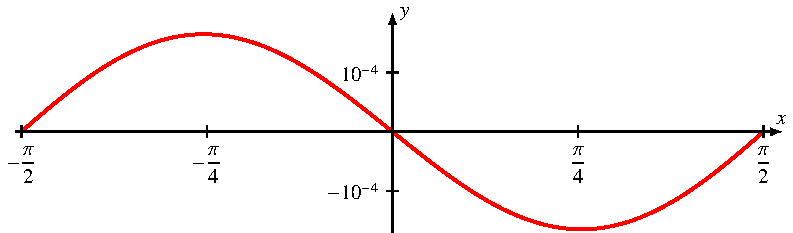
\includegraphics{chapters/30-interpolation/uebungsaufgaben/3001fehler.pdf}
\caption{Fehler des Interpolationspolynoms für $\sin x$ mit Stützstellen
$\frac{\pi}2k$ mit ganzzaligen $k$ mit $-10\le k\le 10$
(Übung~\ref{3001}).
\label{buch:uebungsaufgaben:figure:3001}}
\end{figure}%
\begin{figure}
\centering
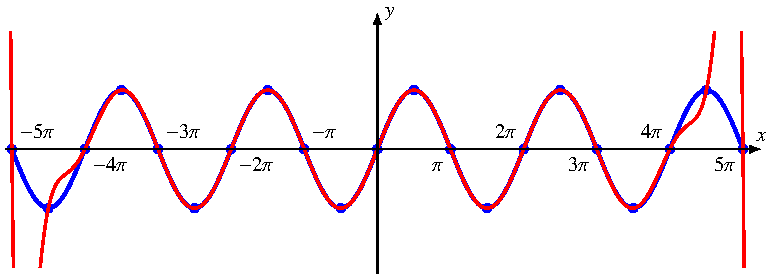
\includegraphics{chapters/30-interpolation/uebungsaufgaben/3001plot.pdf}
\caption{Graph des Interpolationspolynoms für $f(x)=\sin x$ mit Stützstellen
$\frac{\pi}2k$ für ganzzahlige $k$ mit $-10\le k\le 10$.
Trotz des grossen Abstandes und der sehr speziellen Wahl der Stützstellen 
folgt das Interpolationspolynom (rot) der Funktion (blau) in der Mitte des
Definitionsbereichs sehr genau.
\label{buch:uebungsaufgaben:figure:3001plot}}
\end{figure}%
In der Tat ist der Fehler viel kleiner als diese Schranke vermuten lässt.
In Abbildung~\ref{buch:uebungsaufgaben:figure:3001plot} kann man
erkennen, dass das Interpolationspolynom die Funktion in der Mitte
des Intervalls sehr genau wiedergeben kann.
Nur am Rande weicht es wegen des Runges Phänomens stark ab.
\index{Runges Phänomen}%
In Abbildung~\ref{buch:uebungsaufgaben:figure:3001} ist der Fehler
$\sin x -p(x)$ für $x\in[-\frac{\pi}2,\frac{\pi}2]$ dargestellt, es zeigt
sich, dass der Betrag des Fehlers kleiner als $1.66\cdot 10^{-4}$ ist.
\end{loesung}

